\section{Google Connector}
\subsection{\emph{gdata}}

\begin{frame}{Die \emph{gdata}-Bibliothek}

\end{frame}

\subsection{Service erstellen}

\begin{frame}[fragile]{Google-Service erstellen (1)}
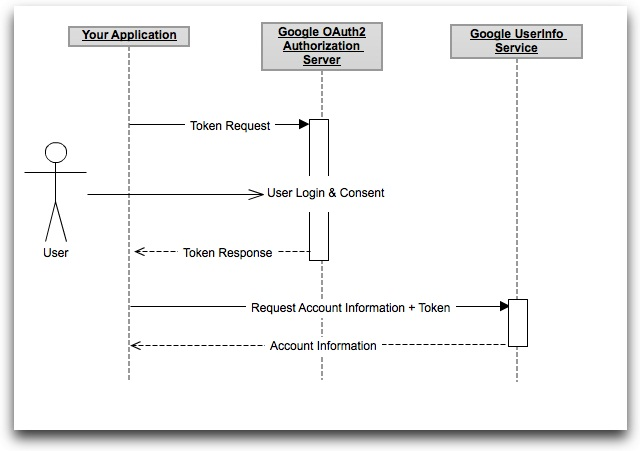
\includegraphics[width=\textwidth]{Bilder/googleOauth.jpg}
\footnote{https://developers.google.com/accounts/docs/OAuth2}
\end{frame}

\begin{frame}[fragile]{Google-Service erstellen (2)}
\begin{block}{Username und Password}
\javalstset
\begin{lstlisting}
ContactsService myService;
myService = new ContactsService(servicename);
try {
	myService.setUserCredentials(username, password);
} catch (AuthenticationException e) {
	e.printStackTrace();
}
\end{lstlisting}
\end{block}
\end{frame}

\subsection{Create Contact}

\begin{frame}[fragile]{Einen Kontakt erstellen (1)}
\begin{block}{Kontakt-Objekt erstellen}
\javalstset
\begin{lstlisting}
// Create the entry to insert
ContactEntry contact = new ContactEntry();
contact.setTitle(new PlainTextConstruct(contactInfoCopy.getFirstname()
		+ contactInfoCopy.getLastname()));
\end{lstlisting}
\end{block}
\end{frame}

\begin{frame}[fragile]{Einen Kontakt erstellen (2)}
\begin{block}{Namen in ein Kontakt-Objekt einfügen}
\javalstset
\begin{lstlisting}
// Name
Name name = new Name();
name.setFamilyName(new FamilyName(contactInfoCopy.getLastname(), null));
name.setGivenName(new GivenName(contactInfoCopy.getFirstname(), null));
contact.setName(name);
\end{lstlisting}
\end{block}
\end{frame}

\begin{frame}[fragile]{Einen Kontakt erstellen (3)}
\begin{block}{Benutzerdefinierte Einträge zu einem Kontakt-Objekt hinzufügen}
\javalstset
\begin{lstlisting}	
// Firma
if (contactInfoCopy.getCompany() != null) {
	ExtendedProperty company = new ExtendedProperty();
	company.setName(DLI_GoogleContactsConnector.company);
	company.setValue(contactInfoCopy.getCompany());
	contact.addExtendedProperty(company);
}
\end{lstlisting}
\end{block}
\end{frame}

\begin{frame}[fragile]{Einen Kontakt erstellen (4)}
\begin{block}{Das Kontakt-Objekt senden}
\javalstset
\begin{lstlisting}
// Kontakt senden		
URL postUrl = new URL(contactsURL);
return myService.insert(postUrl, contact);
\end{lstlisting}
\end{block}
\end{frame}

\subsection{Get Feed}

\begin{frame}[fragile]{Kontakte suchen mit \emph{Queries}}
\begin{block}{Kontakte suchen mit \emph{Queries}}
\javalstset
\begin{lstlisting}
URL feedUrl = new URL("https://www.google.com/m8/feeds/contacts/dli.ides.api@gmail.com/full");
Query myQuery = new Query(feedUrl);
ContactFeed resultFeed = null;
// Gruppe
myQuery.setStringCustomParameter("group", "http://www.google.com/m8/feeds/groups/dli.ides.api%40gmail.com/base/587c880e884cdacb");
// submit request
resultFeed = myService.query(myQuery, ContactFeed.class);
\end{lstlisting}
\end{block}
\end{frame}

\begin{frame}[fragile]{Kontakte holen}
\begin{block}{Kontakte holen ohne \emph{Queries}}
\javalstset
\begin{lstlisting}
URL feedUrl = new URL("https://www.google.com/m8/feeds/contacts/dli.ides.api@gmail.com/full");
resultFeed = myService.getFeed(feedUrl, ContactFeed.class);
\end{lstlisting}
\end{block}
\end{frame}